% Ignorierte Warnings
\RequirePackage{silence}
\WarningFilter{chktex}{You should perhaps use `\min' instead.} % unfortunately -
\WarningFilter{chktex}{You should perhaps use `\max' instead.} % - doesn't work

\documentclass[11pt,twocolumn,abstract=true]{scrartcl}
% Documentclass-options

%%%%% Workarounds %%%%%
\setlength{\marginparwidth}{2cm} % without: trouble with todonotes

\newcommand*\appendixmore{% add title to Abstract
  \addsec{\appendixname}%
  \renewcommand{\thesubsection}{\Alph{subsection}}%
}
%%%%% Workarounds %%%%%

% Debug
%\usepackage{lua-visual-debug}
%\usepackage{endfloat}

% Language-Encoding
\usepackage{polyglossia}        % Alternative zu Babel
\setmainlanguage[variant=british]{english}
\setotherlanguage[babelshorthands=true]{german}


% Citation, Verweise
\usepackage[backend=biber]{biblatex}
\addbibresource{BibLaTex/citavi_db.bib}
\usepackage{csquotes}           % Bei Polyglossia+Babel empfohlen
\usepackage{nameref}
\usepackage{listings}           % Paket zum Einfügen von Source Code.
                                % refer to 'minted vs. texments vs. verbments'
\usepackage{hyperref}

% Fonts
\usepackage{fontspec}
\usepackage{glossaries} % \gls{<golssary-entry>} muss vor unicode-math geladen werden
\setacronymstyle{long-short}
\usepackage{unicode-math} % fontspec wird auch von unicode-math geladen
\setkomafont{disposition}{\normalfont\bfseries}
\setmainfont{TeX Gyre Pagella}
% \setmathfont{TeX Gyre Pagella Math} Somehow faulty with \mathscr
% \setmainfont{Times New Roman} - Unverhältnismäßig hässlich. Besser keine Font
% setzen.


% Sonstiges                     % Einfügen von Grafiken
\usepackage{graphicx}
\graphicspath{ {./pictures/} }
\usepackage{xcolor}
\usepackage[normalem]{ulem}     % Unterstreichen von Text mit \uline
\usepackage{titling}
\usepackage{blindtext}          % Repräsentativer als Lorem Ipsum
\usepackage{kantlipsum}         % Cooler als blindtext
\usepackage{todonotes}          % Einfügen von Todos, Option: [disable]
\usepackage[shortcuts]{extdash} % \=/ for nonbreaking dash
\usepackage{url}

\author{Malte Zietlow, Anna-Lena Büßelmann}
\makeglossaries{}

\begin{document}

\title{Survey: Visual Approaches Towards Interpretability Of Neural Networks}
\maketitle


% Frontmatter
\listoftodos{}            % Aktuelle ToDo-Notes
\begin{abstract}
    \blindtext[1]
\end{abstract}

% Mainmatter
\section{Introduction}
More and more \glspl{nn} are used in the day to day life. \glspl{nn} learn something and then replicate it, but how exactly the internals of the network work is not as easy to find out. Finding a way to communicate in an explainable way how \glspl{nn} compute their output has been a problem ever since. 
\par 
Because of that, many different approaches have been made over the last years. Today there are multiple models, which allow a human to understand a \gls{nn}, like heatmaps or diagrams, which show the most important parts of the input.

\subsection{Structure of this paper}
This paper aims to give a brief overview on the current state of research of visualizing a \gls{nn}. 
\par 
Section 1 describes the methodology of the paper, by defining the target audience and finding criteria for inclusion of research. Thereafter definitions for a heatmap, interpretability and explanation are made in section 2. Next in section 3 the Taxonomy for the following chapters is introduced. Then general concepts for understanding the later explained methods are established.
\par
The methods for visualization are categorized in Gradient-Based Methods, Perturbation-Based Methods and Meta-Methods.
Gradient-Based Methods observe the infinitesimal change in model prediction with respect to a root point \(x_0\) of the predictor \(f\).
Perturbation-Based Methods are based on actually varying the input (by either  perturbation or occlusion) and interpreting the differences in the output.
Meta-Methods use approaches of the other categories and refine them further by combining them oder adding an extra step to the explanation.
\par
Thereafter known issues are addressed.
Finally a conclusion is found and future research is presented.

\subsection{Target audience}
This paper is targeted at an audience that is looking for a theoretical introduction to the field of heatmapping. Knowledge of basic building blocks (such as perceptron, convolutional\=/, recurrent-cells), activation-functions (such as ReLU, tanh), common datasets (such as MNIST, ImageNet), and well known models (such as the VGG-family, AlexNet) is assumed.

\subsection{Criteria for inclusion}
To limit the amount of included research, criteria for inclusion was found. Research which was accepted by a renowned conference or published by a researcher, who is well known for other publications, will be included in this paper. In addition the amount of citations of publications must be significant. Furthermore new research will be mentioned, which was published in the last few months, but not accepted by a conference until now or with just a small number of citations, but shows fundamental new findings.
\section{Background}


\subsection{What is interpretability?}
According to \fcite{Gilpin.2018} “The goal of interpretability is to describe the internals of a system in a way that is understandable to humans”. For this an explanation must be found, that is simple enough and uses meaningful vocabulary for a person. In addition the bias and knowledge must be considered.
\fcite{DoshiVelez.2017} use a similar definition of Interpretability that is adapted to machine learning: Interpretability is “the ability to explain or to present in understandable terms to a human”. \fcite{DoshiVelez.2017} also mentions, that not all ML systems need to be interpretable, because not all systems require human-machine-interaction. 
/par
But especially in today's society, where more and more ML is used, humans want to understand the decisions for safety and ethical reasons. They will not use something they do not understand or trust.
\fcite{DoshiVelez.2017} also mentions, that for knowledge gain a scientific understanding is indispensable.


\subsection{Why is interpretability a necessity?}
\todo{drinbehalten?}

\subsection{What is an explanation?}
There are multiple views on what an explanation actually is. For this paper a scientific definition is chosen. An explanation focuses on explaining the process inside a neural network and answers the question “Why does this particular input lead to that particular output?” \fcite[p.2]{Gilpin.2018}

\subsection{What is a heatmap?} 
For visualizing the decisions of a neural network most researchers are using heatmaps. Heatmaps describe, which parts of the input data are most important for the output. A heatmap can exist in various forms, e.g.\ as a list of objects, which is sorted by relevance or for visual images a image, which shows the most important pixels by color. \fcite{Acona.2018} also mentions, that most often the task of one neuron is researched. Such maps are called attribution maps, in which red and blue markers indicate if the point of data (pixel) contributes positively or negatively to the feature.

\section{Taxonomy}
Visual interpretability of \gls{nn} as discussed in this survey finds itself as a subset of the \textit{explainable artificial intelligence}-research sector. Alternative approaches are rule-extraction\= or intrinsic methods~\cite{ras2018explanation}. The field of visual interpretability itself can be broken into multiple subsets, for example \fcite{vanDerMaaten2008} propose to build a mapping of latent-represantations of input-samples via dimensionality reduction onto a 2D-Plane. However, in this work we are mainly concered with generating heatmaps (\cref{subsect:heatmap}) for input-samples. We distinguish between Gradient-Based and Perturbation-Based methods, which we found to dominate the literature in this area of research.

\subsection{Gradient-Based} Gradient-Based approaches generate heatmaps by observing the change in model-output \(f(x)\) with respect to an input-variable \(x_i\). In this subsection, the set of gradient-based approaches will be further split into~\ref{itm:function},~\ref{itm:signal}, and~\ref{itm:attribution} approaches. 
\subsubsection{Functions, Signal and Attribution} In the past years, a large variety of gradient-based methods have been proposed (e.g.~\cite{Bach.2015,Zeiler.2014,Springenberg.2015,Kindermans.2018,Lundberg.2017,Gurumoorthy.2017,Simonyan.2014,DanielSmilkov.,Sundararajan.2017,Landecker.2013,Zhang.2018,Shrikumar.,Selvaraju.2017}). Broadly speaking, each method explains either~\ref{itm:function},~\ref{itm:signal}, or~\ref{itm:attribution}~\cite{Kindermans.2018,Kindermans.2019}. Usually, this is done by \textit{projecting} the model-output \(f(x)\) back into the input-space \(\mathbb{R}^{|x|}\) of input-sample \(x\), with \(x\in \mathbb{R}^{|x|}\).
\begin{description}
    \item[\namedlabel{itm:function}{Function}{}] approximates the amount by which an infinitesimal change in each dimension (in the following: \textit{variable}) \(i\) in the input-sample \(x\) influences the model-output \(f(x)\). The strength and direction are then simply the partial derivative with respect to the input-variable \(x_i\), i.e.\ \(\frac{\partial f(x)}{\partial x_i}\). However, as function-approaches are usually considered to be only poorly informatory~\cite{Kindermans.2018} and are only used as a baseline, they will not be detailed in this work. For details, please refer to, for example, \fcite{Simonyan.2014}.
    \item[\namedlabel{itm:signal}{Signal}{}] tries to reveal which input-variables caused the prediction~\cite{Kindermans.2018,Zeiler.2014} Signal-approaches are, to the best of our knowledge, constrained to \glspl{cnn}. Signal-approaches include for example DeConvNet~\cite{Zeiler.2014} and Guided Backpropagation~\cref{subsect:guided-backprop}, which have been shown to only approximate patterns that cause increased neuron-activity in higher layers~\cite{Kindermans.2019} (i.e.\ layers close to the output-layer). A more recent approach to this is PatternNet~\cref{subsect:patternnet-attribution}
    \item[\namedlabel{itm:attribution}{Attribution}{}] tries to approximate the contribution of each input-value \(x_i\in x\). This is usually called either \textit{attribution} or \textit{relevance}. Approaches to this are SHAP~\cite{Lundberg.2017}, ProtoDash~\cite{Gurumoorthy.2017}, \gls{lrp} \cref{subsect:lrp}, \gls{td} \cref{subsect:td}, \gls{dtd} \cref{subsect:dtd}, and PatternAttribution \cref{subsect:patternnet-attribution}.
\end{description}

\subsection{Perturbation-Based}
Not only Gradient-Based, but many Perturbation-Based methods were developed in the last years (\cite{AmitDhurandhar.2018,Ribeiro.2018,Luss.,Kim.2018,Zintgraf.2017}). They visualize how parts of the input data correspond with certain features and which influence they have on the given output. This is done by altering the input in certain ways and measuring the differences. Results are visualized in either a diagram (Prediction Difference Analysis: \cref{subsect:PDA}, Anchors: \cref{subsect:anchors}) or a heatmap (LIME: \cref{subsect:lime}). Some methods like LIME (\cref{subsect:lime}) are even able, to work with text as well as pictures and can present their results in both, diagrams and heatmaps. 
\par
The Contrastive Explanations Method (\cref{subsect:CEM}) uses an own approach and visualizes \glspl{pp} and \glspl{pn}. What these are is explained later. Activation Maximization (\cref{subsect:ActivationMax}) computes an input for a certain feature, that activates the feature the most, here the output is an image.
\section{General Concepts}
\blindtext[3]
\subsection{Types of Explanation}
\blindtext[3]

\subsection{Axioms}
Following the terminology of~\cite{Sundararajan.2017}, axioms describe desirable properties which a method should satisfy.

\subsubsection{Conservativity}
\blindtext[1]
\subsubsection{Continuity}
\blindtext[1]
\subsubsection{Explicitness}
\citeauthor{AlvarezMelis.2018}
\blindtext[1]
\subsubsection{Stability}
\citeauthor{AlvarezMelis.2018}
\blindtext[1]
\subsubsection{Diversity}
\citeauthor{AlvarezMelis.2018}
\blindtext[1]
\subsubsection{Grounding}
\citeauthor{AlvarezMelis.2018}
\blindtext[1]
\subsubsection{Implementation Invariance}
\blindtext[1]
\subsubsection{Selectivity/Fidelity}
`Put another way, a method with high fidelity will assign high relevance to features that, when removed, greatly reduce the DNN’s output confidence in the class assignment, while assigning low relevance to features that do not greatly affect the confidence when removed. Fidelity cannot be established axiomatically, and so must be estimated using implementations of the explanation method with the DNN model and dataset under investigation.'\cite{Tomsett.2019} Also look up: \citeauthor{Bach.2015, AlvarezMelis.2018}.

\subsection{Sanity Checks for Saliency Maps}
\blindtext[1]

\subsection{Metrics}
Although the field of heatmapping has received growing attention over the past decade, only little work has gone into the development of metrics. This is an issue, because absence of ground truth makes the search for metrics a non-trivial task --- while the lack of (reliable) metrics leads to flaws in the comparison of methods.

This subsection will provide a theoretical overview of commonly used metrics, \cref{metrics:aopc,metrics:faithfulness,metrics:roar}. Tools for verifying the reliability of metrics are given in~\fullref{metrics:sanity-checks}. A final overview and discussion are presented in~\fullref{metrics:discussion}

\subsubsection{Area Over the Perturbation Curve}\label{metrics:aopc} Proposed by~\citeauthor{WojciechSamek.2015}~\cite{WojciechSamek.2015}, \gls{aopc} is a generalization of the \textit{pixel flipping method} presented in~\cite[pp. 34ff.]{Bach.2015}. \gls{aopc} measures the degradation of model-score for a certain input-sample, as input-variables are disabled in an iterative manner. Following either \gls{morf} or \gls{lerf} order. \gls{morf} and \gls{lerf} are extracted from the set of locations \[ \mathscr O = (\symbfit{r}_1, \symbfit{r}_2, \dots, \symbfit{r}_L), \] \todo{consider factoring this out as a general concept} which is ordered by decreasing relevance, i.e.\ informally: \[(i > j) \implies \text{relevance}(\symbfit{r}_i) < \text{relevance}(\symbfit{r}_j) \] Here, a location \( \symbfit{r}_p, p \in [1, L] \) must not be a single input, but could represent any constant multidimensional array of inputs (e.g.\ a \( 9\times9 \)-grid of pixels, as seen in the original paper).

\paragraph{Disabling Input Variables}
Disabling input variables comes with the risk of violating dataset statistics such as mean and variance. A sample-perturbation function that disables the region \(\symbfit{r}_k\) in the input-sample \(\symbfit{x}\) is formally introduced as \(g(\symbfit{x}, \symbfit{r}_k)\). \citeauthor{WojciechSamek.2015} propose to four sample-perturbation functions
\begin{itemize}
    \item replacing each value in \(\symbfit{r}_p\) by sampling a uniform distribution \(\mathscr U\)
    \item replacing each value in \(\symbfit{r}_p\) by sampling a Dirichlet distribution \(D\)
    \item replacing each value in \(\symbfit{r}_p\) by the average value of all samples for the current input-variable
    \item applying a Gaussian filter with \(\sigma = 3\) to \(\symbfit{r}_p\)
\end{itemize}
Note that the latter two, Gaussian filter and average value for the current input-variable, remove significantly less information from the input-sample than sampling from either \(\mathscr U\) or \(\mathscr D\).  Therefore (as removing information from the input-sample is the goal of disabling input variables) \citeauthor{WojciechSamek.2015} favor the first two, i.e.\ sampling \(\mathscr U\) or \(\mathscr D\).


\paragraph{Most Relevant and Least Relevant First}
\gls{morf} (eq1 and eq2) and \gls{lerf} (eq3 and eq4) are both defined recursively \todo{Correctly reference equations}
\begin{align}
    \symbfit{x}^{(0)}_{\text{MoRF}} &= \symbfit{x} \\
    \forall{1 \leq k \leq L}: \symbfit{x}^{(k)}_{\text{MoRF}} &= g(\symbfit{x}^{(k-1)}_{\text{MoRF}}, \symbfit{r}_k) \\
    \symbfit{x}^{(0)}_{\text{LeRF}} &= \symbfit{x} \\
    \forall{1 \leq k \leq L}: \symbfit{x}^{(k)}_{\text{LeRF}} &= g(\symbfit{x}^{(k-1)}_{\text{LeRF}}, \symbfit{r}_{L+1-k})
\end{align}
where \(x^{(n)}_{\text{MoRF / LeRF}}, n \in [0, k]\) is the perturbed input-sample\todo{add \textit{input-sample} to glossary} at iteration \(n\) and by the respective order \gls{morf} / \gls{lerf}.

\paragraph{Area Over the Perturbation Curve}
The \gls{aopc} is then defined as
\[
    \text{AOPC}_M = \dfrac{\left< \sum_{k=0}^{L} f(\symbfit{x}^{(0)}_{M}) - f(\symbfit{x}^{(k)}_{M}) \right>}{L+1},
\]
where \(\left< \cdot \right>\) denotes the average over all input-samples\todo{define input-sample globally} in the \mbox{data set} and \(M \in \{\text{MoRF}, \text{LeRF}\}\). Informally, \gls{aopc} calculates the arithmetic mean of the average decrease in model-score\todo{define model-score globally. Model-score is more like model output, actually.} caused by disabling a range from \(0\) to \(L\) input variables\todo{define input variable globally}.

\subsubsection{Faithfulness}\label{metrics:faithfulness}
For faithfulness~\cite{AlvarezMelis.2018, Tomsett.2019}, as opposed to~\nameref{metrics:aopc}, model-outputs are computed with only a \textit{single} input-variable\todo{define input-variable globally} disabled at a time. Faithfulness is computed by taking Pearson correlation between the drop in model-output (when disabling the input-variable) and the relevance assigned to the input-variable by the heatmapping-method. Formally, given a sample \(\symbfit{x}\) with \(\left|\symbfit{x}\right|=n\) input-variables, an input-variable \(i\in \symbfit{x}\), the sample \(\symbfit{x}_i\) where \(i\) is disabled, a drop in model-output \(\Delta_i\) and a relevance for the input-variable \(R_i\):
\begin{align*}
    \Delta_i = f(\symbfit{x}) - f(\symbfit{x}_i)\\
    \text{Faithfulness}_{\symbfit{x}} = \frac{1}{n}*\rho(R_i, \Delta_i)
\end{align*}
gives the Faithfulness for a single image \(\symbfit{x}\). The Faithfulness over the full dataset is computed as
\[
    \text{Faithfulness} = \left<\rho(R, \Delta)\right>
\]
where, again, \(\left< \cdot \right>\) denotes the average over all input-samples in the \mbox{data set}


\subsubsection{Remove And Retrain}\label{metrics:roar}
\blindtext[3]

\subsubsection{Sanity Checks for Metrics}\label{metrics:sanity-checks}
Just as for heatmaps, sanity checks were proposed for metrics~.\cite{Tomsett.2019} For determining whether a metric \textit{measures the intended property} and \textit{provides consistent results}, \citeauthor{Tomsett.2019} build upon three psychometric reliability tests (notice that both~\ref{itm:inter-rater} and~\ref{itm:inter-method} assume a \textit{fixed} metric)
\begin{description}
    \item[\namedlabel{itm:inter-rater}{Inter-rater reliability}] measures if heatmapping-methods are ranked consistently over the set of all input-samples.
    For calculation, \citeauthor{Tomsett.2019} refer to Krippendorff's \(\alpha\).
    \begin{description}
        \item[\(\alpha = 1\)] implies that a metric assigns the same ranking-order for the heatmapping-methods (i.e.\ if a heatmapping method is superior, it is consistently superior). 
        \item[\(\alpha = 0\)] implies that a metric assigns a random score for each heatmapping-method. Therefore, the fidelity of a heatmapping method cannot be predicted using the observed metric.
    \end{description} \todo{Read this again}
    \item[\namedlabel{itm:inter-method}{Inter-method reliability}] measures the correlation of metric-scores for different heatmapping methods over the set of all input-samples. For calculation, \citeauthor{Tomsett.2019} refer to Spearman's \(\rho\). A large \(\rho\) implies high inter-method reliability.
    \item[Internal consistency] measures if different metrics observe the same property (e.g.\ fidelity). For calculation, \citeauthor{Tomsett.2019} take the correlation (again, Spearman's \(\rho\)) of metric-scores from different metrics over the same heatmap.
\end{description}

\subsubsection{Discussion}\label{metrics:discussion}
\blindtext[1]

\section{Gradient-Based Methods}
\blindtext[3]

\subsection{Deconvolution}
\blindtext[3]
\subsection{Guided Backprop}
\blindtext[1]
\subsection{Layer-Wise Relevance Decomposition}
\blindtext[3]

\subsubsection{Taylor-Decomposition}
\blindtext[3]

\subsubsection{Deep-Taylor-Decomposition}
\blindtext[3]
\subsection{LIFT}
\blindtext[3]
\subsection{PatternNet and PatterAttribution}\label{subsect:patternnet-attribution}
Using either a simple linear model~\cite{Kindermans.2018} or a constant shift in mean~\cite{Kindermans.2019}, \citeauthor{Kindermans.2018} were able to show the vulnerability of gradient methods (such as \gls{lrp}, \gls{td}, \gls{dtd}, Gradient x Input, and Integrated Gradients) to random changes in the input-sample (see \cref{fig:kindermans-unreliability}).
\begin{figure*}
    \center{}
    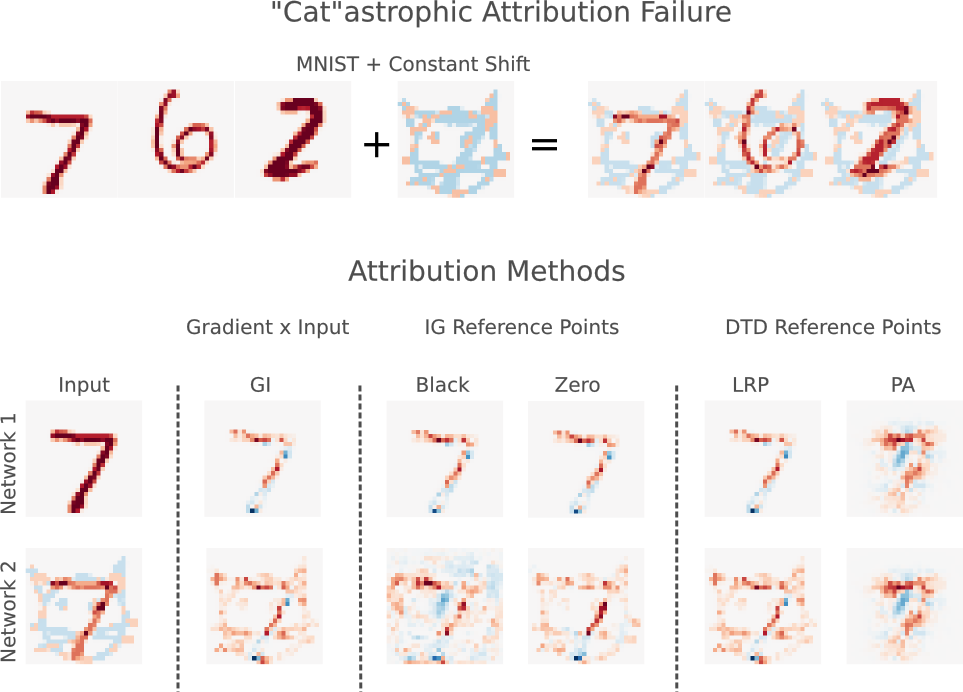
\includegraphics[width=\textwidth]{kindermans-catastrophic-attribution}
    \caption[Evaluation of attribution methods via a constant shift on MNIST]{Evaluation of attribution methods on two models (Network 1 and Network 2). Network 1 is trained on the well known MNIST-Dataset, while Network 2 is trained on a manipulated Version of MNIST with a constant shift (i.e. a hand-drawn image of a cat). Because the constant shift does not add any information to an image, a consistent attribution method should provide a similar explanation for both Network 1 and Network 2, when applied to the same input image with only the constant shift. However, Gradient x Input, Integrated Gradients and \gls{lrp} show a difference between Network 1 and Network 2. For further details, refer to~\cite{Kindermans.2019} from where this figure was adopted.}
    \label{fig:kindermans-unreliability}
\end{figure*}
To overcome this vulnerability of preexisting methods, \fcite{Kindermans.2018} introduce \textit{signal estimators} \(S(x)\) that will be explained in this subsection. Signal estimators root in the idea that each input-sample \(x\) of a dataset is a combination of underlying signal \(s\) (contains all information about e.g.\ the correct class) and distractor \(d\) (does not contain any information about e.g\ the correct class) such that \(x=s\circ d\), with \(\circ\) being some operation, for simplicity let \(\circ\) denote summation \(\circ:=+\)~\cite{Kindermans.2018}. A signal estimator \(S(x)\) is then used to extract \(d\) from \(x\), such that for an optimal signal estimator: \(s = x - S(x)\).
\begin{description}
    \item[\namedlabel{itm:sw-signal-estimator}{The Filter-Based Estimator \(\symbfit{S_w}\)}{\(\symbfit{S_w}\)}] is equal to the \ref{itm:w2weighting} discussed in \cref{subsect:dtd}.
    \begin{equation}
        S_w = \frac{w_{ij}^2}{\sum_{h\in (l)} w_{hj}^2}.
    \end{equation}
    Although simple, \fcite{Kindermans.2018} show that \(S_w(x)\) neither holds theoretically, being unable to separate \(s\) and \(d\), nor empirically as shown in \cref{fig:kindermans-signal-estimator-comparison}.
    \item[\namedlabel{itm:sa-signal-estimator}{The Linear Estimator {}\(\symbfit{S_a}\)}{\(\symbfit{S_a}\)}] is based on the assumption of a linear perceptron. Although this assumptions does not even hold for simple ReLU's, it provides a significant improvement over \ref{itm:sw-signal-estimator} as shown in \cref{fig:kindermans-signal-estimator-comparison}.
    \begin{equation}
        S_{a(i)}(x) = x_{(i)} (a_{(i)} w_{ij})\label{eq:linear-estimator}
    \end{equation}
    please note that, while the weights \(w_{ij}\), which are taken from a trained model, and the input-variable of the input-sample \(x_{(i)}\) are fixed parameters, \(a_{(i)}\) must be trained on a given dataset. Details on the training are provided in~\cite{Kindermans.2018}. \Cref{eq:linear-estimator} is an exemplary formulation of \(S_a\) for the input layer.
    \item[\namedlabel{itm:sa+-signal-estimator}{The Two-Component Estimator \(\symbfit{S_{a+-}}\)}{\(\symbfit{S_{a+-}}\)}] is tailored to ReLU-activation functions. \fcite{Kindermans.2018} notice that due to applying ReLU's, the weights used in previous signal estimators \ref{itm:sw-signal-estimator}, \ref{itm:sa-signal-estimator} are only trained on positive signal \(s_{+}\) and distractor \(d_{+}\) values. To account also for negative \(s_{-}, d_{-}\), they split the estimator accordingly
    \begin{equation}
        S_{a+-(i)} = 
        \begin{cases}
            x_{(i)} (a_{+(i)} w_{ij}),& {\scriptstyle \text{if } (x_{(i)} w_{ij}) > 0}\\
            x_{(i)} (a_{-(i)} w_{ij}),& {\scriptstyle \text{otherwise}}
        \end{cases}
    \end{equation}
    again note that, while the weights \(w_{ij}\) and the input-variable \(x_{(i)}\) are fixed parameters, \(a_{+(i)}, a_{-(i)}\) must be trained on a given dataset. Details on the training are provided in~\cite{Kindermans.2018}.
\end{description}\label{desc:signal-estimators}
\par
In summary, \citeauthor{Kindermans.2018} propose 
\begin{enumerate*}[label={\roman*)}]
    \item the concept of signal estimators in order to overcome the vulnerability of previous methods to a constant-shift in the input and
    \item two new signal estimators, \ref{itm:sa-signal-estimator} and \ref{itm:sa+-signal-estimator}, which significantly improve upon the previously (and naively) used estimator \ref{itm:sw-signal-estimator}.
\end{enumerate*} A visual example for the three signal estimators is provided in \cref{fig:kindermans-signal-estimator-visually}.
\par
For \textit{PatternAttribution}, \fcite{Kindermans.2018} then use the derived signal estimator as a weighting parameter in the \gls{dtd}-framework, which can be interpreted as an informed choice of root-point \(x_0\).
For \textit{PatternNet}, only the signal itself is reconstructed.% \todo{sHOw aN iMaGE oF THiS}
\begin{figure*}[ht]
    \center{}
    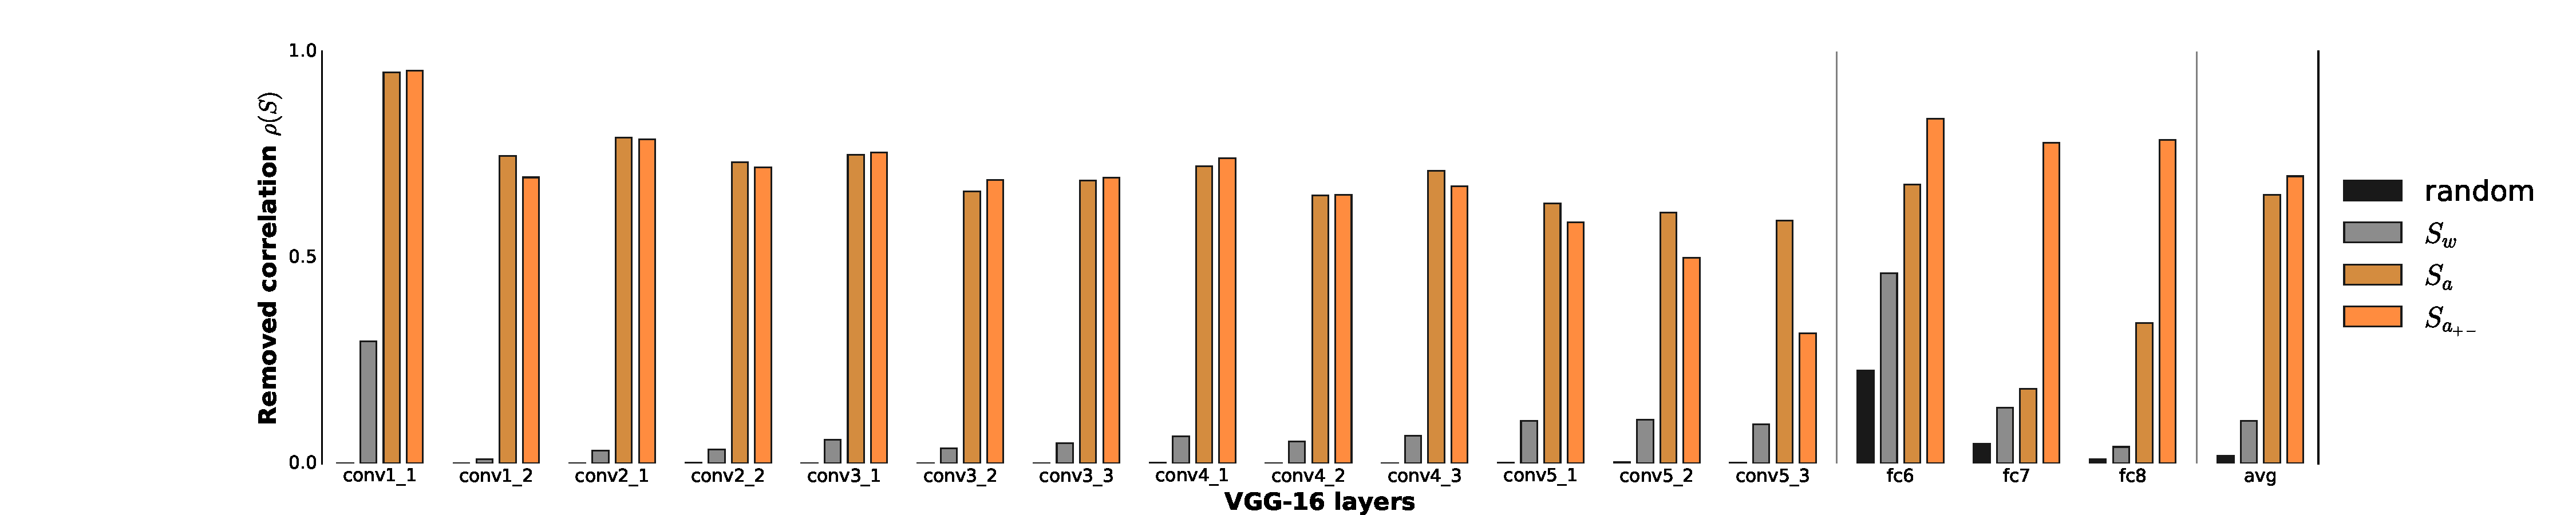
\includegraphics[width=\textwidth]{kindermans-signal-estimators}
    \caption[Evaluation of Signal Estimators for VGG-16 on different layers.]{Evaluation of Signal Estimators for VGG-16 on different layers. Higher values are better. A random Signal Estimator is used as baseline. For details on the quality measure \(\rho\) refer to \cite{Kindermans.2018} from where this figure was adopted.}
    \label{fig:kindermans-signal-estimator-comparison}
\end{figure*}
\begin{figure}
    \center{}
    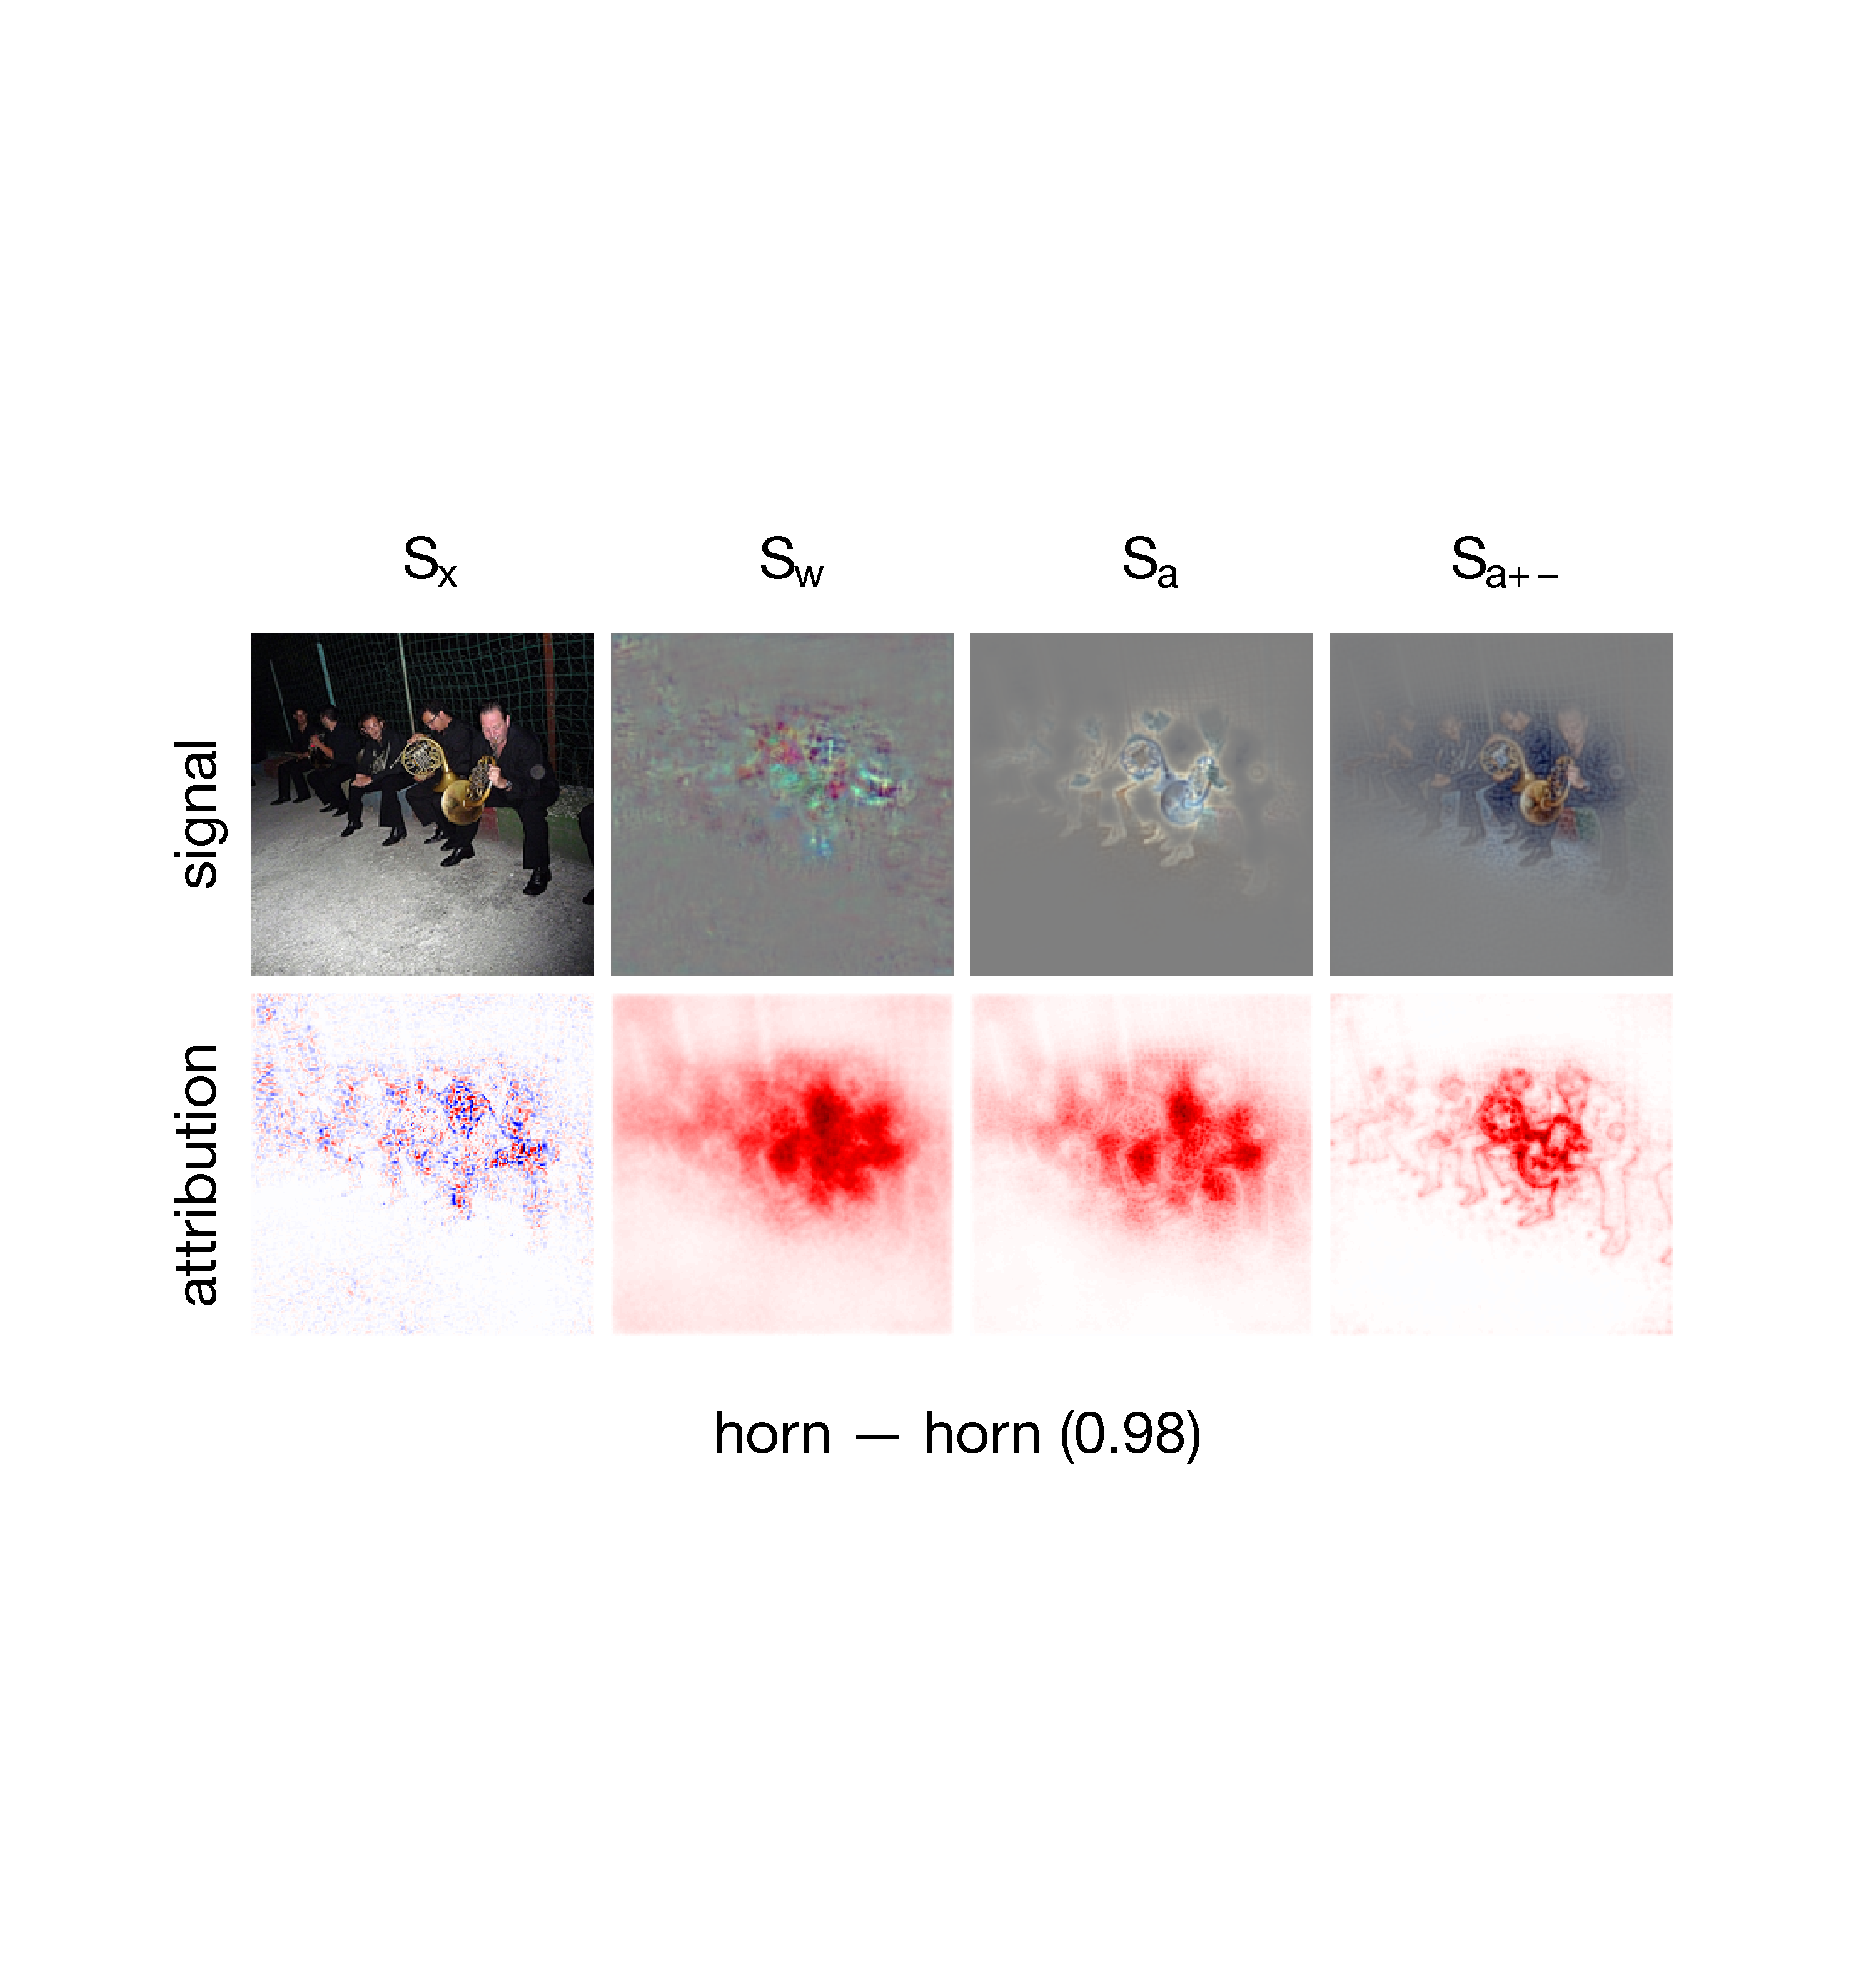
\includegraphics[width=\textwidth/2]{kindermans-signal-estimators-visually}
    \caption[Visual example for the three signal estimators.]{Visual example for the three signal estimators. \(S_x\) is the identity estimator with \(S_x(x)=x\). Figure adopted from~\cite{Kindermans.2018}}\label{fig:kindermans-signal-estimator-visually}
\end{figure}
\subsection{ProtoDash}
\blindtext[1]
\subsection{SHAP}
\blindtext[3]

\section{Perturbation-Based Methods}
Perturbation based methods for Visualizing NNs are methods, which compute “the attribution of an input feature (or set of features) by removing, masking or altering them, and running a forward pass on the new input, measuring the difference with the original output” \cite[2]{Acona.2018}.
These methods “allow a direct estimation of the marginal effect of a feature” (\cite[p.2]{Acona.2018}), but do not achieve the needed performance when it comes to a higher number of features.
\par
Because of this, there are many new approaches in this field.
Various methods are based on perturbation of input data. In this meta study the focus will be on Prediction Difference Analysis, but multiple other methods will be mentioned and and the current state of research will be explained.


\subsection{LIME}
LIME is another Algorithm that aims to explain the predictions of a NN and is short for “Local Interpretable Model-agnostic Explanations”. It was first introduced by \fcite{Ribeiro.2016} and is freely accessible at https://github.com/marcotcr/lime.
\par
It is applicable to different types of data, like pictures and text and computes the most relevant features of this input. For a picture LIME would output the relevant parts of a picture, for a text the decisive words in some form of diagram. The explainers correspond with the actual explanation at 90 to 97\%. Multiple examples will be seen in this paper and compared to other methods \cite{Ribeiro.2016}.

\subsection{Occlusion Methods}
Occlusion Methods, otherwise known as Input Masking or Representation Erasure, alter the input by concealing certain parts of the input data and measuring the difference in the output compared to the original output. 
\par
\fcite{Li.2016} use this method for word embeddings. They mask the Pre- or Suffix or other Dimensions of a word and calculate the difference in the output. Like this, the most important dimensions can be found. Interestingly erasure of certain words returns an negative importance score, this means, it improves the decision of the network \cite{Li.2016}.

\subsection{Contrastive Explanations Method CEM}
The \glspl{cem} was first published by \fcite{Dhurandhar.2018} in 2018 in their paper “Explanations based on the Missing: Towards Contrastive Explanations with Pertinent Negatives”.
The \gls{cem} approach aims to identify the minimal amount of pixels to justify a classification, called \glspl{pp}. On the other hand side it identifies the pixels as well, that need to be “turned off” in order to change the classification of the image. These pixels are called \glspl{pn}. Like this, the most important pixels can be found \fcite{Luss.}. 
\par
“For example, when justifying the classification of a handwritten image of a 3, the method will identify a subset of non-zero or on-pixels within the 3 which by themselves are sufficient for the image to be predicted as a 3 even if all other pixels are turned off (that is, made zero to match background). Moreover, it will identify a minimal set of off-pixels which if turned on (viz. a horizontal line of pixels at the right top making the 3 look like a 5) will alter the classification” \cite[2]{Luss.}.
This example is visualized in \cref{fig:CEM_Numbers} \cite{Dhurandhar.2018}.
For the algorithm \fcite{Dhurandhar.2018} found formulas to calculate such PPs and PNs.
\begin{figure*}[h]
    \center
    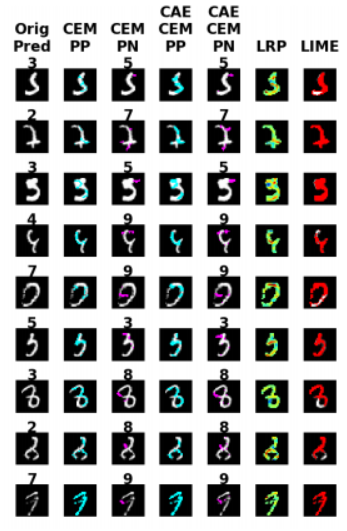
\includegraphics[width=\textwidth/2]{CEM_Numbers}
    \caption{CEM, LRP and LIME applied to a number dataset, \cite{Dhurandhar.2018}}
    \label{fig:CEM_Numbers}
\end{figure*}
They applied this method to a dataset of handwritten numbers, like seen in the example \cref{fig:CEM_Numbers}. They trained a NN, which finally reached an accuracy of 99.4\% and then used \gls{cem} to visualize these decisions. 
\par 
In addition they used a a convolutional autoencoder for some results, which improves this method even further. In \cref{fig:CEM_Celebs} the output of \gls{cem} is visualized. 
\par
To be able to better see the improvements made by this method, LIME and LRP were applied to the same celebrity dataset. It can clearly be seen, that \gls{cem}'s results are better understandable for humans.
\begin{figure*}[h]
    \center
    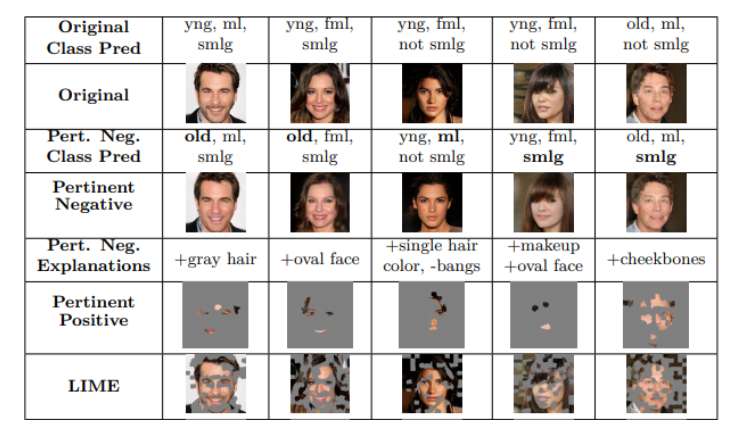
\includegraphics[width=\textwidth]{CEM_Celebs.png}
    \caption{CEM and LIME applied to a celebrity dataset, \cite{Luss.}}
    \label{CEM_Celebs}
\end{figure*}

\fcite{Luss.} improved this method in 2019 and made it applicable to RGB images.
They found, that “For colored images, PPs offer better direction as to what is important for the classification versus too much direction of LIME (shows too many features) or too little direction by Grad-CAM (only focuses on smiles), while for gray-scale images, neither PPs, LIME, or Grad-CAM are particularly informative versus PNs.” \fcite[p.7]{Luss.}

\subsection{Prediction Difference Analysis}
The Prediction Difference Analysis was developed 2008 by \fcite{RobnikSikonja.2008} and published in the paper “Explaining Classifications for Individual Instances”. They address 3 different types of explanation: instance explanation, model explanation and domain explanation. Instance explanation aims to explain a “classification of a single instance at model level” \cite[2]{RobnikSikonja.2008}. Model explanation measures the averages of explanations over multiple instances and can provide a more general explanation of features and the importance of features values.
\par
Domain explanation is still unknown, but “if the accuracy of the model is high, it should be quite similar to the model explanation.” \cite[2]{RobnikSikonja.2008} Firstly they define a model as a function \(f : x \rightarrow f(x)\) which maps instances to numerical values. To calculate the prediction Difference some definitions must be made: An instance x has a value for each attribute \(A_{i}\). To now calculate the effect of Ai on x they observe the models prediction for  \(f(x \backslash A_{i})\). 
\par
If there is just a minor difference the influence of \(A_{i}\) is small, if there is a major difference the influence is large. The defined formula is: 
\(predDiff_{i} (x) = f(x)− f(x \backslash A_{i})\).
\par
The difference can be evaluated as 
\par
    information difference
    \par
        \begin{multline}
              infDiff_{i}(y|x) = \\
              \log_{2} p(y|x)−\log_{2} p(y|x \backslash A_{i})
        \end{multline}
        \par      
    weight of evidence
    \par
        \begin{align}
            \begin{split}
                odds(z) ={}& \frac{p(z)}{p(\bar{z})} = \frac{p(z)}{(1 − p(z)}
            \end{split}\\
            \begin{split}
                WE_{i}(y|x) ={}& \\
                & \log_{2} (odds(y|x)) \\
                & - \log_{2}(odds(y|x \backslash A_{i}))    
            \end{split}
        \end{align}
        \par
    difference of probabilities (output classes)
    \par
        \begin{multline}
            probDiff_{i} (y|x) = \\
        p(y|x)− p(y|x \backslash A_{i})
        \end{multline}
        
\par
The simplest way of computing \(p(y|x \backslash A_{i})\) is to replace the value of the attribute \(A_{i}\) with a special but unknown value, knowing, that this approach can lead to incorrectness if the modeling technique does not handle unknown values naturally (naive Bayesian classificator).
To not depend on the model's implementation they chose an approach, that “simulates the lack of information about \(A_{i}\) with several predictions”\cite[p.4]{RobnikSikonja.2008}.
\par
For  nominal attributes they replace the actual value \(A_{i} = a_{k}\) with all possible values for \(A_{i}\) and weight the prediction by the prior probability of the value: 
\par
        \begin{multline} 
            p(y|x \backslash A_{i}) = \\ 
            \sum_{s=1}^{m_{i}} p(A_{i} = a_{s} | x \backslash A_{i})p(y|x \leftarrow A_{i} = a_{s})
        \end{multline}
        \par
    
        \begin{multline}
            p(y|x \backslash A_{i}) = \\ 
            \sum_{s=1}^{m_{i}} p(A_{i} = a_{s})p(y|x \leftarrow A_{i} = a_{s})
        \end{multline}
        \par

It should be kept in mind, that different instances predict different values, so the explanation differs from instance to instance. Additionally the explanation is dependent on the model, so if the model is incorrect, the explanation will reflect that. The same goes for class dependency, different classes will lead to different explanations.
\begin{figure*}[h]
    \center
    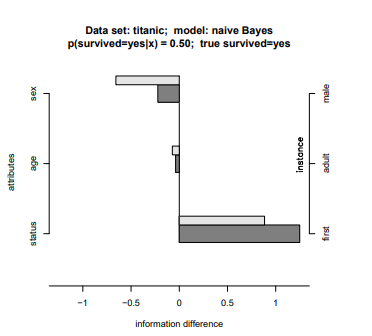
\includegraphics{PDA-Diagram}
    \caption{Prediction Difference Analysis on Titanic-dataset, \cite{RobnikSikonja.2008}}
    \label{fig:PDA-titanic}
\end{figure*}
The results of the prediction difference can then be visualized in a diagram. This special method is called explainVis. \Cref{fig:PDA-titanic} is based on the Titanic dataset and predicts the probability of survival of the person based on travelling class, age and gender.
\par
The information difference is shown on the horizontal axis. Weight of evidence and difference of probabilities produce similar graphs and explanations but differ in scale. On the vertical axis the name of the attribute can be found on the left side and the values for chosen instances on the right side. The class probability 
\(p(y|x)\)
 which was calculated by the model is reported on the top.
The length of the dark grey bar corresponds to the influence of the feature according to the information difference. Positive influence is given on the right-hand side and negative on the left-hand side. The light grey bar represents the influence across all instances for the corresponding attribute value. This shows the overall trend for the feature.
\par
\fcite{Zintgraf.2017} refined this approach even further. They found, that removing one feature at a time is not enough, because a complex neural network is robust to just one unknown feature, like a pixel in an image. Therefore multiple features should be removed at a time so see an impact. In \cite{Zintgraf.2017} they are using images to demonstrate this. They choose patches of connected pixels as their feature sets. The patches have a size of k x k pixel or for an rgb image k x k x 3. Because they use a sliding window style the patches overlap, which makes it possible, to define the individual pixels impact. Depending on the size of the window different results can be found 
\par
It is visible, that a small window does not show the intended results. On the other hand a large window leads to a blurry and not clearly understandable image as well. Therefore observing the results and varying the window size is necessary .like it can be seen in \cref{fig:PDA} (\cite{Zintgraf.2017}). 
\begin{figure*}[h]
    \center
    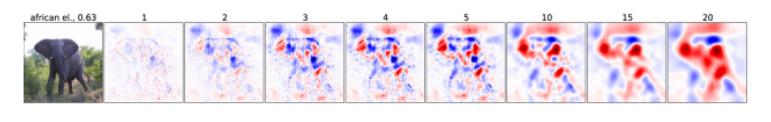
\includegraphics[width=\textwidth]{PredictionDifferenceAnalysis}
    \caption{Prediction Difference Analysis with different window sizes, \cite{Zintgraf.2017}}
    \label{fig:PDA}
\end{figure*}

\subsection{Anchors}
Anchors were introduced in 2018 by \fcite{Ribeiro.2018} and can also be referred as if-then rules. They are rules, that “sufficiently “anchors” the prediction locally – such that changes to the rest of the feature values of the instance do not matter” \cite[1]{Ribeiro.2018}. This means, the values of other features are not important if an anchor exists, because the prediction will always be the same. In their paper they apply these anchors to tabular, text and image datasets.
\par
Like in the prediction difference analyses the model is defined as  
\(f(x) \rightarrow y\). 
An instance x ist perturbed by a “perturbation distribution” \(D_{x}\) (from now on D). The perturbations D should be in an interpretable form. A is a set of rules, which is applicable on x. \(A(x)\) returns true (1), if all feature predicates are true for instance x.
If 
\(A(x) = 1\)
 and “A is a sufficient condition for \(f(x)\) with high probability” \cite[2](Ribeiro.2018) (bigger than τ), then A is an anchor. Formally this can be described with 
\par
\(E_{D(z|A)} [\mathbb{1}_{f(x)=f(z)}] ≥ τ, A(x) = 1\)
 \par
An example of anchors for texts can be seen in figure 5. What LIME is, is explained in section “LIME”. In \cref{fig:Anchor} you can see possible Anchors: e.g. for anchor A = {“not”, “bad”} the model will predict “positive “ with a probability of more than τ. If one or more of these words are missing, there is no anchor and with that it is not certain, what the output will be.
The paper presents two different ways for finding those anchors: a bottom-up construction or a Beam-Search.
\begin{figure*}[h]
    \center
    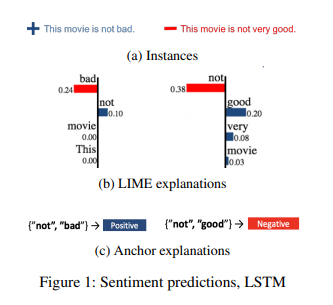
\includegraphics[width=\textwidth/2]{Anchor}
    \caption{possible Anchors for textual data, \cite{Ribeiro.2018}}
    \label{fig:Anchor}
\end{figure*}
\par
With the bottom up search they try to find a rule with the highest estimated precision, and like this the shortest anchor. This anchors tend have a high coverage and are easily understandable for humans. 
The downside of this approach is, that this greedy strategy is only able, to find one anchor at a time and the coverage is just negligibly.
The beam search aims “to identify amongst many possible anchors the one that has the highest coverage” \cite[5]{Ribeiro.2018}. This is done similar to the greedy approach. First all candidate rules are computed, then the best rules are selected.

\subsection{Activation Maximization}
Activation Maximization aims to find an input, which maximizes the output score for a certain class. It was first published in a technical report by \fcite{Erhan.2009} in 2009. They restricted themselves to find the image of the dataset they had, that maximizes the feature.
\par
\fcite{Le.2012} refined this approach in 2012 and not only found the input images with the highest stimuli, but were able to compute an own picture (picture) \cite{Le.2012}.
\par
There are multiple frameworks that can generate such pictures. A well-known method was developed by Zeiler and Fergus in 2014 called DeConvNet \cite{Zeiler.2014}. They mapped features to pixels, instead of the other way around:
“To start, an input image is presented to the convnet and features computed throughout the layers. To examine a given convnet activation, we set all other activations in the layer to zero and pass the feature maps as input to the attached deconvnet layer. Then we successively (i) unpool, (ii) rectify and (iii) filter to reconstruct the activity in the layer beneath that gave rise to the chosen activation. This is then repeated until input pixel space is reached.” \cite[820]{Zeiler.2014}.
\par
\fcite{Nguyen.2016} achieved this in 2016 by starting from a random image and calculating via backpropagation how each pixel influences the output. Multiple studies have shown, that this can lead to unrealistic images. To improve in this point a general concept of a natural image must be learned by the NN. Therefore Nguyen et al. are using image generator networks. They conclude, that they can understand better, which features a NN has learned exactly with this method \cite{Nguyen.2016}. 
\par
In \cref{fig:ActivationMax} the learned feature “face” is demonstrated. On the upper half the actual input images are shown, which activate the neuron the most. On the bottom the generated image is shown.
\begin{figure*}[h]
    \center
    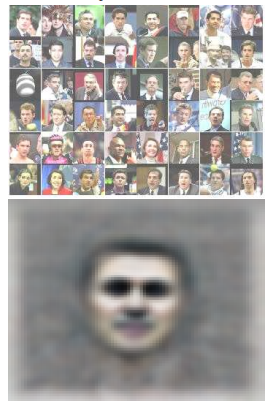
\includegraphics[width=\textwidth/2]{ActivationMaximization}
    \caption{Inputs, that activate the “face-neuron” the most.
    Top: actual input images 
    Bottom: via backpropagation found input, \cite{Le.2012}}
    \label{fig:ActivationMax}
\end{figure*}
\section{Meta Methods}
Meta Methods are using other methods to calculate their results, e\.g\. they can use pre generated heatmaps as an input.

\subsection{Network Dissection}
This method was introduced in 2017 by \fcite{Bau.2017} and is only applicable on convolutional networks. Their methods is divided into three steps: 
“
\begin{enumerate}
    \item  Identify a broad set of human-labeled visual concepts. 
    \item Gather hidden variables’ response to known concepts.
    \item Quantify alignment of hidden variable−concept pairs
\end{enumerate}
” \cite[2]{Bau.2017}
A human interpretable concept is often displayed by a combination of multiple variables and not only one. Nonetheless the paper measures the alignment between a single unit and a single interpretable concept. 
They did this, by finding pictures, that maximize the activation of a feature and then found the part of the picture, all of the pictures had in common (\cref{fig:NetworkDissection} figure 7).
\begin{figure*}[h]
    \center
    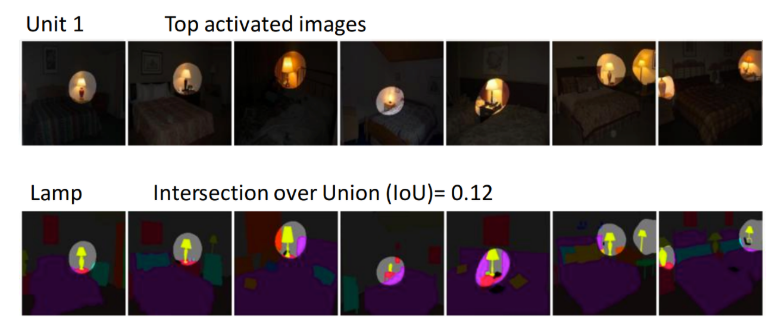
\includegraphics[width=\textwidth]{NetworkDissection}
    \caption{Network Dissection, \cite{Bau.2017}}
    \label{fig:NetworkDissection}
\end{figure*}

Interestingly they found, that lower layers of a CN interpret concepts like color or texture and higher layers more complex concepts like part or object, much like the human way of interpretation \cite{Bau.2017}.

\subsection{Concept Activation Vectors}
Concept Activation Vectors were published by \fcite{Kim.2018} in 2018. It aims to improve heatmaps in the point, that is it is only applicable to one picture at a time. The problem with that is, that even if a picture is of the same object, different parts of the object can be highlighted in the heatmap. This leads to confusion and mistrust.
\par
Their method measures the activation of a layer l produced of certain inputs. They then define a “concept activation vector” (or CAV) as the normal to a hyperplane separating examples without a concept and examples with a concept in the model’s activations” \cite[3]{Kim.2018}.
\par
A concept can be a special feature of a photo, e.g. a striped texture. So to compute such CAV, analysts needs a set of photos of striped objects and a set of random photos.
“Then, a binary linear classifier can be trained to distinguish between the layer activations of the two sets 
[...].
This classifier 
[...]
is a linear CAV for the concept” \cite[3]{Kim.2018}. Like this it can be found, which features exactly a NN learned.
In the paper they used a maximization technique in addition to sort the photos. Like this, the  underlying concept of a CAV can be visualized \cite{Kim.2018}.

\subsection{Spectral Relevance Analysis}
The \gls{spray} was first published in 2019 by \fcite{Lapuschkin.2019}. It aims to combine multiple explanations into one. It applies spectral clustering to pre generated heatmaps and identifies recurrent patterns. 
\par
“The identified features may be truly meaningful representatives of the object class of interest, or they may be co-occurring features learned by the model but not intended to be part of the class, and ultimately of the model’s decision process. Since SpRAy can be efficiently applied to a whole large-scale dataset, it helps to obtain a more complete picture of the classifier behavior and reveal unexpected or ‘Clever Hans’ type decision making” \cite[8]{Lapuschkin.2019}.
\par
\gls{spray} consists of four steps:
\begin{enumerate}
    \item The relevance maps for the dataset need to be calculated.
    \item Thereafter the relevance maps need to be resized to be in a uniform form.
    \item Spectral cluster analysis must be applied to the relevance maps. This groups classifier behaviors into clusters.
    \item Then interesting clusters can then be found via eigengap analysis.
\end{enumerate}
After that the results can be visualized \cite{Lapuschkin.2019}.

\section{Findings}
just to see how long the paper is

\section{Conclusion}
Interpretability of \glspl{nn} is a necessity for various reasons. This paper summarized multiple methods, that aim to visualize these explanations. Since first methods were introduced in \cite{RobnikSikonja.2008} many new approaches have evolved. Some of the most promising methods like \gls{cem} or \todo{was sind denn die interessantesteten sahcxen bei dir?} have found new, but much more interpretable ways of explaining \glspl{nn}. 
\par
Even though there still is no favorable method at this time and for most approaches much more research is necessary, there are more ways than ever to visualize \glspl{nn}.

\section{Future Research}
There have been many new approaches towards Perturbation-Based Methods in the last years. Methods like anchors or \gls{cem} are promising, but need more research in order to refine them and make them applicable to various types of data. 
\todo{ergänzen}


% Backmatter
\appendix

\section{Basic Concepts}
\blindtext[1]

\section{Algorithms of related work}
\blindtext[2]

\section{Concepts of Bounding Box Encoding}\label{append:Concepts of Bounding Box Encoding}
\blindtext[3]



\section{K-Means Clustering}\label{append:K-Means Clustering}
\blindtext[3]%~\cite[386-390]{James.2017}
\section{Bounding Box Offsets}
\blindtext[1]

\section{Preprocessing}
\blindtext[3]

\section{Concepts of Neural Network Architectures}
\blindtext[3]
\subsection{Convolutional Layer}\label{append:Convolutional Layer}
% receptive field~\cite[335-345]{IanGoodfellow.2016}
\blindtext[1]
\blindtext[3]

\section{Loss Functions}
\blindtext[2]

\section{VGG16 and ResNet (Base Networks)}
\blindtext[3]


%\chapter{General Todos}

% Consider colophon  
%% You’re recommended to use the eprint-aware biblio styles which
%% can be obtained from e.g. www.arxiv.org. The file mythesis.bib
%% is derived from the source using the SPIRES Bibtex service.
\onecolumn{\printbibliography{}}  %% Literaturverzeichnis
\printglossaries{}      % Glossar
%% I prefer to put these tables here rather than making the
%% front matter seemingly interminable. No-one cares, anyway!
\listoftables           % Tabellenverzeichnis
\listoffigures          % Abbildungsverzeichnis

% ----------------------------- Acronyms -----------------------------
\newacronym{aopc} {AOPC} {Area Over the Perturbation Curve}
\newacronym{abpc} {ABPC} {Area Between the Perturbation Curves}
\newacronym{morf} {MoRF} {Most Relevant First}
\newacronym{lerf} {LeRF} {Least Relevant First}
\newacronym{roar} {ROAR} {Remove And Retrain}
\newacronym{kar} {KAR} {Keep And Retrain}
\newacronym{lrp} {LRP} {Layer-wise Relevance Propagation}
\newacronym{td}{TD}{Taylor-Decomposition}
\newacronym{dtd}{DTD}{Deep-Taylor-Decomposition}
\newacronym{pp} {PP} {Pertinent Positive}
\newacronym{pn} {PN} {Pertinent Negative}
\newacronym{ai} {AI} {Artificial Intelligence}
\newacronym{nn} {NN} {Neural Network}
\newacronym{cnn}{CNN}{Convolutional Neural Network}
\newacronym{spray}{SpRAy}{Spectral Relevance Analysis}
\newacronym{cem}{CEM}{Contrastive Explanations Method}

% ----------------------------- Glossary Entries -----------------------------

\newglossaryentry{path}{
    name={path},
    description={A path \(P_{i, j}\) exists between two neurons \(i, j\) if the value of \(i\) is fed into \(j\).},
}

\newglossaryentry{message}{
    name={message},
    description={Messages are defined in \fullref{subsubsect:message-notation}}
}




\end{document}